%%%%%%%%%%%%%%%%%%%%%%%%%%%%%%%%%%%%%%%%%%%%%%%%%%%%%%%%%
%%%%%%%%%%%%%%%%%%% author:hijeffery %%%%%%%%%%%%%%%%%%%%
%%%%%%%%%%%%%%%%%%% part:14.0-14.6   %%%%%%%%%%%%%%%%%%%%
%%%%%%%%%%%%%%%%%%%%%%%%%%%%%%%%%%%%%%%%%%%%%%%%%%%%%%%%%

\chapter{自编码器}
\label{chap:14}

\emph{自编码器}是神经网络的一种,用以训练来实现将输入复制到输出的目的。在其内部,有一个用编码表示输入的隐层$h$。自编码器可以看作由两部分组成:编码函数$h = f(x)$ 和进行信号重建的解码函数$r = g(h)$。 具体结构如图\ref{fig:14.1}所示。如果自编码器学到的结果仅仅是处处将$g(f(x)) = x$,则其没有起到任何作用。相反,自编码器被设计成了不能够完美的复制输入到输出的工作方式。通常他们被限定在只能够近似的复制,并且只复制能够与训练数据相像的输入。鉴于模型被强制执行输入的某些部分应当被复制,所以通常来讲,自编码器能够学习到数据的有用的特性。


\begin{figure}[htbp] %  figure placement: here, top, bottom, or page
   \centering
   \includegraphics[width=1in]{fig/chap14/14.1.png} 
   \caption{自编码器的基本结构,将输入信号$x$通过一个内部表征或者编码$h$ 映射到输出(也叫重建) $r$。 自编码器有两个子部分:编码器(将$x$映射到$h$)与解码器(将$h$映射到$r$)。}
   \label{fig:14.1}
\end{figure}

现代自编码器已经从执行特定的函数映射扩展到了执行随机映射$p_{encoder}(h|x)$ 和 $p_{decoder}(x|h)$。

自编码器的思想已经在神经网络研究领域存在了几十年。传统上来讲,自编码器是用来执行数据降维与特征学习的。近来,自编码器与隐变量模型的联系使得自编码器成为生成模型的研究前沿,详情见本书第\ref{chap:20}章介绍。自编码器可以视为前馈网络的一种特殊形式,并且可以用与其相同的方式进行训练,如以子集沿着反向传播计算的梯度下降方向求解。同一般的前馈网络不同的是,自编码器也可以用\emph{再循环}的方式进行训练,即对比原始输入的网络相应与重建信号作为输入的网络相应的差别。再循环技术被视为比反向传播算法更为接近生物特性的方法,但是其很少被出现在其他机器学习应用中。

\section{不完备自编码器}
将输入复制到输出听起来似乎无特别作用,但其实我们也不关心解码器的输出。事实上,我们期望通过训练自编码器实现复制输入的任务能够产生有实用意义的$h$。

一个从自编码器获取有效的特征的方法是将$h$限定到一个比$x$更低的维度上。特征维度比输入维度低的自编码器是\emph{不完备}的。学习一个不完备的特征迫使自编码器捕获到训练数据中的最为突出的特征信息。

学习过程可以简单的表述为最小化一个随时函数的形式:
\begin{equation}
	L(x,g(f(x)))
\end{equation}
其中,损失函数 $L$ 通过如最小化均方误差等限定$g(f(x))$ 与 $x$ 尽量相近。 

当解码器是线性函数,并且$L$ 是均方误差时,不完备自编码器学习到的生成子空间与PCA一致。此时,被用来执行复制任务的自编码器事实上附加学到了训练数据的主子空间。

因此,具有非线性编码函数$f$和非线性解码函数$g$的自编码器可以学习到更强有力的非线性泛化PCA。遗憾的是,如果编码与解码部分被给予太强能力的化,自编码器仍然仅仅完成复制输入到输出的功能而忽略了抽取数据分布等有效信息的能力。理论上说,我们可以设想一个只有一维编码的自编码器,其编码器具有强大的能力将每一个训练数据$x^{(i)}$表示成编码$i$。此外,解码器能够学习并将每一个整型值映射回特定的训练数值上。这种特殊情形在现实中不会出现,但其足够说明,一个被训练用来进行数据复制的自编码器,如果被赋予了过与强大的能力,并不会学习到任何与用的信息。


\section{用自编码器进行流行学习}
\label{sec:14.6}

同其他很多机器学习方法一样,自编码器同样假设数据集中在一个低维流面或者一个这种流面的小集合上,详见\ref{sec:5.11.3}节。一些机器学习方法效果有限,尽管他们可能可以学习到一个在流面上正常的函数,但是对于不在流面上的输入,可能会产生不正常的表现。
自编码器进一步拓展了这种思想,并设法去学习流行的结构。

为了理解为什么自编码器能够有这样的效果,我们需要介绍流行的几个重要的特性。

其中一个很重要的特性是其\emph{正切平面}集合。对于一个d-维流面上的点$x$, 其切面是由能够张成流面上局部方向变化的d-维向量给出。如图\ref{fig:14.6}所示,这些局部方向指出了我们能如何对$x$在流面上进行无限小的位置改变。
\begin{figure}[htbp] %  figure placement: here, top, bottom, or page
   \centering
   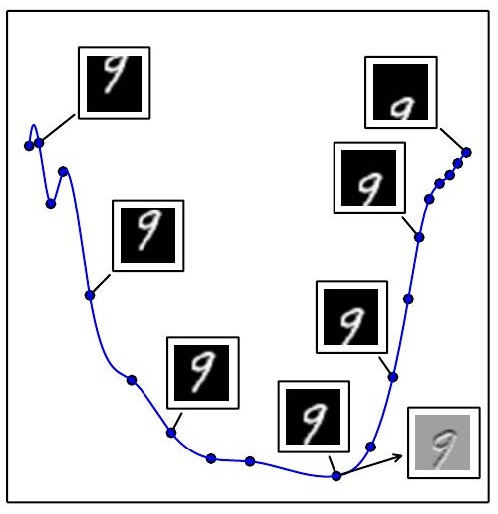
\includegraphics[width=4in]{fig/chap14/14_6.jpg} 
   \caption{超切平面概念示意图。这里我们给出一个784-维空间内的一维流面。我们选取MNIST数据集中的一幅784像素的图像,并沿着竖直方向移动它。这样的一组竖直移动数据定义了沿一维流面方向的坐标,并在图像空间中划出一条曲线。图中给出了在这个流面上的几个点。为了可视效果,我们用PCA把流面投影到了二维空间中。一个n维流面在任一点都有一个n维切面。切面在流面上的该点处完美贴合,并且与该点的表面平行。该切面定义了使得数据保持在流面上的可以移动的方向空间。图中的一维流面有一个单独的切线。我们在图中给出了一个切线示例,以及在图像空间中沿切线移动时所产生的变化。灰色的像素是在移动过程这个不发生变化的点,白色代表颜色变亮,黑色代表颜色加深。}
   \label{fig:14.6}
\end{figure}

所有的自编码器的训练过程是两个限定因素的折衷:

1. 学习一个训练样本$x$的特征表示$h$,使得$x$能够通过解码器从$h$中大致恢复出来。$x$是从训练样本抽取的这个事实使得问题有点儿麻烦,因为这意味着自编码器没有必要对与不在数据生成分布下的输入进行很好的重建。

2. 满足限定或者泛化惩罚。这个可以是结构上限定自编码器的容量的设定,或者是添加到重建误差后的一项泛化项。这些技术通常倾向于对于输入数据不敏感的解决方案。

显然,不管是从输入到输出的复制本身,或者是直接忽略输入,二者任何之一单独出现都没有太大作用。相反,二者同时出现,能够保证方法有效,因为他们迫使隐藏特征表示去捕获能够描述数据生成分布的内在结构。重要的一点就是自编码器可以只去表示重建训练数据所必须的那些变化。如果生成数据的分布本身集中在一个低维流面上,这诱使特征描述仅仅表现这个流面上的一个局部的坐标系统:即只有在$x$附近的与流面相切的变化可以联系到$h = f(x)$的改变上。所以,自编码器学到的从输入空间$x$到表示空间的映射,是一个仅仅对于在流面方向上的变化敏感但对于垂直于流面方向上的变化不敏感的映射。

图\ref{fig:14.7} 给出了一个一维的例子,该图表明通过限定重建函数对于数据点周围扰动的敏感性,我们的自编码器可以重建流面结构。
\begin{figure}[htbp] %  figure placement: here, top, bottom, or page
   \centering
   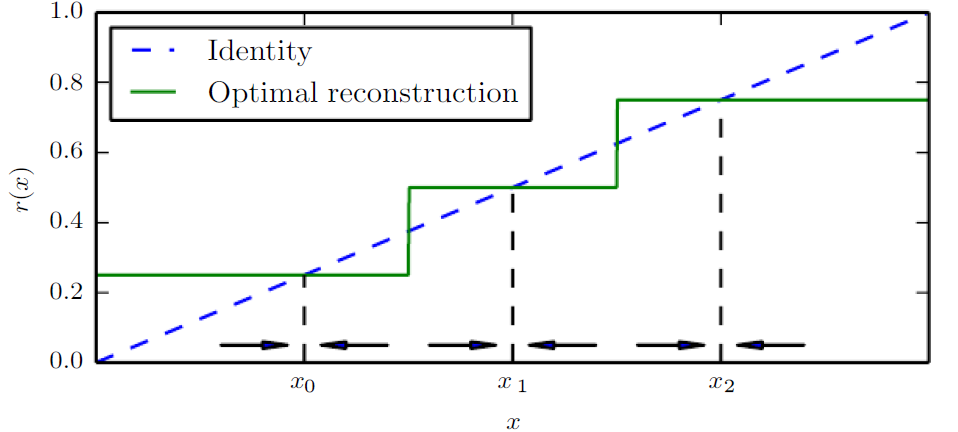
\includegraphics[width=4in]{fig/chap14/14_7.png} 
   \caption{如果自编码器学习到了一个能够对在数据点周围的扰动具有不变性的重建方程,则其学习到了数据本身的流行结构。图中给出的是0-维流面的流行结构。虚线表示用以重建的恒等函数。最有重建函数在有数据的地方同恒等函数重合。底部的箭头表示重建误差向量$r(x)-x$,在输入空间,这些箭头总是指向其最近的“流面”(在一维的情况下,是一个孤立点)。降噪自编码器直接设法使重建函数$r(x)$的偏导数在数据点周围尽量小。收缩自编码器对于编码器进行了同样的操作。尽管$r(x)$的导数在数据点周围尽量小,在不同数据点之间,它可以变得很大。数据点之间的空间同流面之间的区域直接相关,在这些地方,重建函数的导数必须很大,才能将被破坏的点重新映射回流面上。}
   \label{fig:14.7}
\end{figure}

为了更好的理解为什么自编码器可以进行流行学习,我们有必要将其与其他方法进行比较 。对于流行的特性最常用的研究方法是点在流面上或者流面附近的\emph{特征表示}。对于某个样本的特征表示也被称作其嵌入。特征表示通常用一个低维的向量来表示,即比作为一个低维子集存在的流面的原始外部空间的维数要低。一些算法直接对每一个训练样本学习一个嵌入表示(如下面导论到的非参数流行学习方法),与此同时,其他的一些方法则设法学习到一个更为通用的映射,该映射将周围空间(输入空间)映射到嵌入空间。有时这种映射被叫做自编码器或者表示方程式。 

流行学习通常关注于非监督学习的方法来得到这些流面。早期的大部分学习流面的研究集中在基于最近邻图模型的非参数方法上。在图模型中,每个样本表示为一个节点,并通过边将最近邻的样本连接起来。如图\ref{fig:14.8}所示,这些方法将每个节点表示为切平面,这些切平面描述了样本同其邻域样本的变化方向。
\begin{figure}[htbp] %  figure placement: here, top, bottom, or page
   \centering
   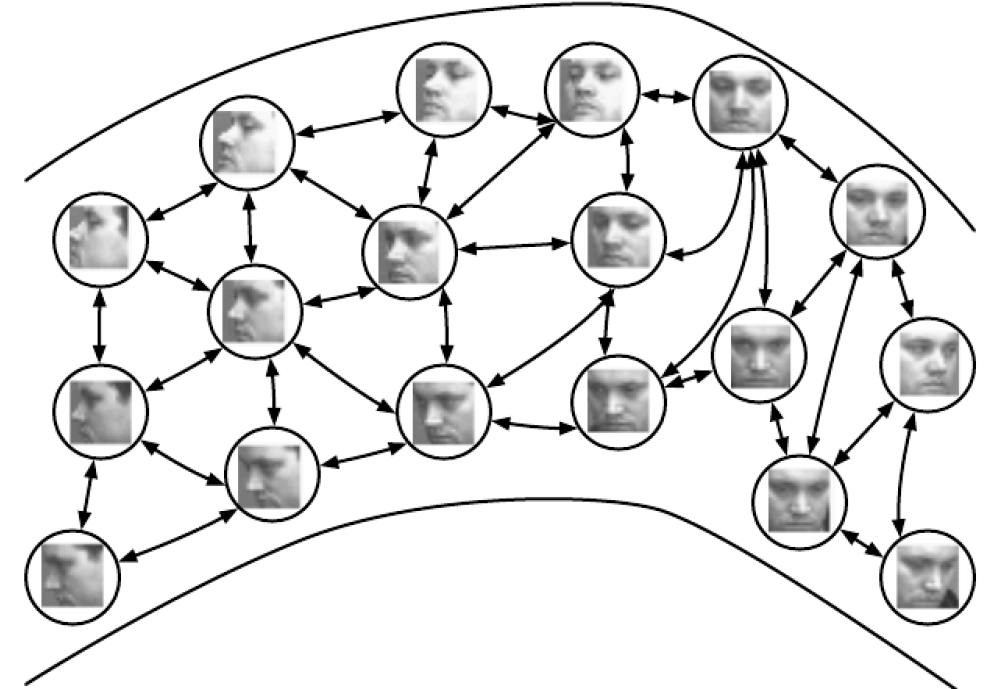
\includegraphics[width=4in]{fig/chap14/14_8.png} 
   \caption{非参数流行学习方法构建了一个最近邻图模型,其中,节点表示训练样本,有向边表明最近邻关系。如此,通过各种不同的方法可以得到切平面以及与其相对应的邻域图模型,此外,还有一个将每一个样本同一个实值向量或嵌入对应的坐标系统。如此我们可以通过一定的改动使特征表示适应新的样本。只要样本数量足够大能够覆盖流面的弯曲与褶皱,这些方法都可以很好的工作。图片来源为QMUL多视人脸数据库。}
   \label{fig:14.8}
\end{figure}

我们之后可通过优化算法或者求解线性系统来获取一个全局坐标系统。图\ref{fig:14.9}给出了一个流面视如何平铺成大量的局部线性类高斯碎片的(或者叫做圆饼,因为高斯函数在切线方向是平坦的)。
\begin{figure}[htbp] %  figure placement: here, top, bottom, or page
   \centering
   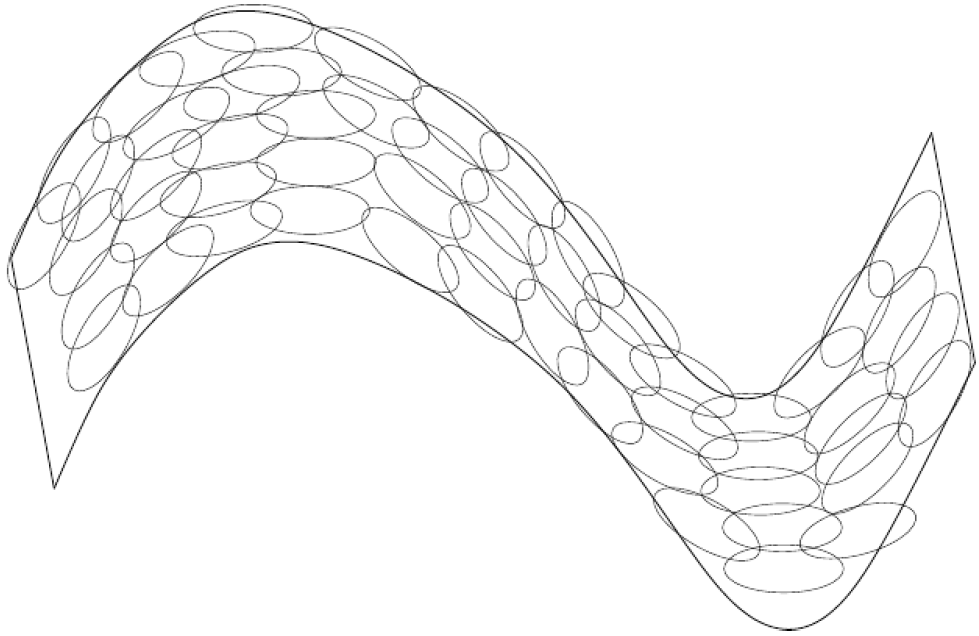
\includegraphics[width=4in]{fig/chap14/14_9.png} 
   \caption{如果切平面(参考图\ref{fig:14.6})在处处都是已知的,则他们可以平铺成一个全局的坐标系统或者密度方程。每一个局部分块都可以被看成是一个局部的欧氏坐标系统或者局部扁平高斯或者圆盘,他们在垂直于圆盘的方向变化很小,在定义圆盘坐标系统的方向上变化很大。这样的一些高斯函数组合成了在流面高斯窗算法或者其基于非局部神经网络的变种中的一个预测密度函数。}
   \label{fig:14.9}
\end{figure}

但是,用这些局部非参数的方法在进行流行学习的时候有一个基本的难题:如果流面本身非常不平整(有许多峰值、低谷、褶皱),我们可能需要大量的样本来覆盖这些变量,从而降低了对未知样本的泛化能力。事实上,这些方法仅仅能够通过邻域信息的插值来泛化流面的形状。不幸的是,在人工智能问题中涉及到的流行往往具有非常复杂的结构,很难从局部插值中获取所有信息。比如说图\ref{fig:14.6}中的通过平移变换产生的流面,如果我们仅仅观察输入向量的一个坐标$x_i$的话,当图像移动时,我们可以看到,每当图像在遇到灰度的峰值或者低谷的时候,我们的坐标就会遇到一个峰值或者低谷。换言之,待处理图像的灰度明暗的复杂度决定了对于像进行简单的平移操作产生的流面的复杂度。这些促使了通过分布式描述和深度学习进行流行结构学习的需求。
